\chapter{Solución planteada}
\section{Descripción general}

En este proyecto se desarrolla una aplicación para la edición y ejecución de un espectáculo de \emph{video mapping} que se denomina \emph{Video Mapping Tool (VMT)} la cual está basada en los enfoques anteriormente descriptos: bidimensional y tridimensional.
Esta aplicación dispone de un editor tridimensional en el cual se importan modelos en formatos específicos permitiendo visualizarlos desde distintos puntos de vista mediante cámaras virtuales. De forma análoga permite la creación de objetos bidimensionales para generar así un modelo mixto, adaptable a las distintas necesidades de los usuarios.

Para la producción del espectáculo, \emph{VMT} brinda distintos efectos como la proyección de imágenes, videos y degradado de colores, los cuales se pueden aplicar de igual forma a objetos bidimensionales y tridimensionales. A su vez existen efectos específicamente para objetos tridimensionales que permiten variar su posición en el tiempo.
\emph{VMT} brinda una línea de tiempo sobre la cual es posible definir el orden de ejecución de estos efectos, mediante su asociación a un instante del espectáculo. A su vez también es posible especificar la ejecución de efectos desencadenados por eventos de teclado o \emph{MIDI}.
Mediante el editor que brinda \emph{VMT}, es posible asociar una pista de audio que acompañará al espectáculo.

La aplicación tiene la capacidad de utilizar múltiples proyectores, permitiendo así cubrir una amplia superficie. El resultado de estas proyecciones puede ser previsualizado de forma centralizada en el editor, logrando visualizar desde diferentes ángulos los efectos aplicados sobre el modelo.
La calibración de la proyección es asistida por \emph{VMT} mediante distintos mecanismos para objetos bidimensionales y tridimensionales utilizados en la escena.

La persistencia del espectáculo se logra almacenando y cargando la definición del mismo desde archivos \emph{XML} estándar.

\emph{VMT} es una aplicación multiplataforma de código abierto, basado en \emph{OpenFrameworks}\cite{openframeworks} y \emph{Qt Framework}\cite{QT} que permite su compilación y ejecución en entornos \emph{Microsoft Windows}, \emph{Linux} y \emph{Mac OS X}.

\section{Funcionalidades}

\subsection{Manejo de escena}

Una escena en \emph{VMT} es una colección de objetos, efectos y cámaras que serán representados gráficamente.
Se cuenta con un motor de dibujado que se encarga de generar dicha representación brindando soporte a la visualización de elementos gráficos bidimensionales y tridimensionales en pantalla o proyectados. También brinda el soporte para el mapeo de texturas de imágenes o videos sobre estos objetos.
Este motor ofrece una interfaz para el manejo y edición de objetos y efectos que contiene la escena.

Los elementos bidimensionales manejados por \emph{VMT} son cuadriláteros que en el contexto de la aplicación se denominan \emph{quads}. Éstos se pueden posicionar en pantalla de forma tal que al ser proyectados cubran una superficie total o parcial de la escena. Luego, sobre estos \emph{quads} se aplicarán texturas en forma de imagen o video, para que la proyección deforme estas texturas adaptándolas a la forma del \emph{quad}.
Los \emph{quads} también pueden ser utilizados como máscaras para cubrir zonas en donde no se desee proyectar. Esto puede ser útil cuando se desea proyectar sobre una superficie con forma compleja en la que un \emph{quad} no se adapta a la sección deseada. Una máscara se logra con un \emph{quad} opaco de color negro ya que este color es el menos visible al ser proyectado.

Los elementos tridimensionales representan objetos más complejos y ofrecen una mayor versatilidad para realizar mapeos sobre ellos.
El formato utilizado para representar los elementos tridimensionales es \emph{3DS}\cite{3DS} por lo cual es posible cargar al motor cualquier geometría que lo respete.
La edición de la geometría de estos objetos tridimensionales es en general un tema complejo que lo resuelven varias aplicaciones de edición tridimensional entre ellas \emph{3D Studio}\cite{3DStudioMax} y Blender\cite{Blender}. Por esta razón es que se delega la edición de las formas tridimensionales a programas para este propósito.
Los programas de edición además de permitir modificar la geometría manipulando vértices y caras, también posibilitan la definición de materiales para aplicar propiedades comunes a una cierta selección de caras de la malla tridimensional$^\dagger$.
\emph{VMT} utiliza estas selecciones de caras para mapear texturas sobre ellas resolviendo de esta forma el mapeo en tres dimensiones. Este mapeo es controlado mediante la definición de coordenadas \emph{UV} en cada vértice del modelo. Las aplicaciones de edición tridimensional antes mencionadas proveen herramientas para hacer esta tarea de forma intuitiva. Ejemplo de esto es la definición de coordenadas de mapeo a un cilindro para mapear una textura en una columna cilíndrica.

En \emph{VMT} los elementos gráficos por sí mismos no son representables, siendo necesario asignarles un material y es a éste al que se le asigna un color o una textura con la cual se representará el objeto.
En la implementación de los materiales se utilizan \emph{shaders} que son programas que se ejecutan en los procesadores gráficos y tienen como ventaja ser altamente paralelizables, permitiendo realizar cálculos de forma rápida y eficiente. En la aplicación se utiliza el lenguaje de \emph{shaders} \emph{GLSL}\cite{GLSL} para \emph{OpenGL} para la implementación de un \emph{shader} básico que combina una textura de imagen o video con un color, obteniendo así el resultado final del material. Este color tiene un canal alfa$^\dagger$ que permite representar texturas y colores con distintos niveles de transparencia.

Para visualizar los elementos tridimensionales es necesario definir un punto de vista. Esto se logra mediante la utilización de una cámara virtual y la configuración de sus propiedades, entre ellas su ubicación y orientación. Los proyectores con los que se realiza el espectáculo de \emph{video mapping} son también representados como cámaras, aunque no toda cámara virtual representa un proyector, ya que es posible contar con cámaras adicionales que representen puntos de vista de interés para el usuario como por ejemplo el de un observador del espectáculo.
Las cámaras permiten ajustar sus parámetros de forma similar a otros paquetes de animación por software y a cámaras cinematográficas en general. Estas operaciones representan movimientos de la cámara llamados \emph{Roll}, \emph{Orbit}, \emph{Dolly} y \emph{Pan}.
\emph{Roll} se refiere al movimiento en donde la posición de la cámara y el punto de vista son fijos y ésta rota a través del eje formado por ellos.
\emph{Orbit} es cuando la cámara orbita alrededor de su punto de vista, es decir, la posición de la cámara cambia pero siempre visualizando el mismo punto y manteniendo la distancia a este.
\emph{Dolly} es el movimiento en donde se mantienen el punto y la dirección de vista pero se mueve la posición de la cámara acercándose o alejándose del objetivo.
Por último, \emph{Pan} es el tipo de movimiento en el cual se mueve la cámara manteniendo un paralelismo con la dirección de vista, cambiando la posición y el punto de vista.

\begin{figure}[H]
  \centering
    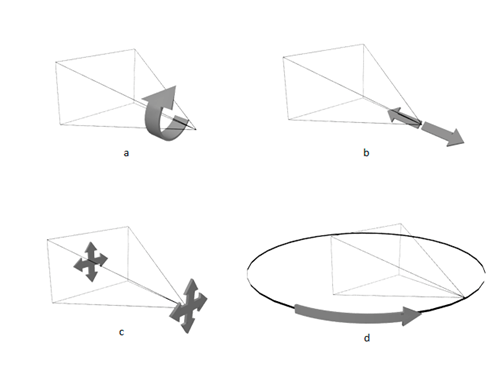
\includegraphics[width=0.5\textwidth]{./Cap5_vmt/vmtengine-cameramove.png}
  \caption[Imagen propia.]{Movimientos de cámara. a) \emph{Roll} b) \emph{Dolly} c) \emph{Pan} d) \emph{Orbit}}
  \label{fig:VMT-CameraMove}
\end{figure}

Además de estos parámetros de ubicación, también existe el parámetro \emph{Field Of View (FOV)} o campo de vista que es el ángulo de apertura de la cámara. Para el caso de cámaras que representan proyectores, este parámetro debe coincidir con el ángulo de apertura del proyector para ajustar correctamente las escenas con respecto a lo que muestra la cámara en pantalla.
Mediante estas operaciones es que las cámaras virtuales de \emph{VMT} ajustan sus parámetros para que la proyección de objetos tridimensionales coincida con las superficies proyectadas.
Hay que destacar que las cámaras proveen un punto de vista únicamente para los elementos tridimensionales. Los \emph{quads}, que como se mencionó, son construcciones bidimensionales, no dependen del punto de vista de la cámara y se representan en un sector de la pantalla relativo a ésta. Es por esto que los \emph{quads} no alteran su posición en pantalla al ajustar los parámetros de la cámara.

Los \emph{quads} se pueden organizar en grupos que a su vez se organizan en una o más capas. Cada capa pertenece a una única cámara de manera de representar las zonas a cubrir por un solo proyector. Es posible aplicar una transformación inicial a una capa, la que se aplicará a todos los \emph{quads} o grupos de \emph{quads} contenidos en ella. Esto es útil para ajustar la proyección de los \emph{quads} en caso de mover el proyector levemente y que esta proyección deje de coincidir con las superficies, lo cual provee la funcionalidad básica y de bajo nivel para el mecanismo de calibración bidimensional que se detallará más adelante.

Las texturas se asocian a grupos de \emph{quads} que permiten variar la manera en que se mapean las texturas a los \emph{quads} que los componen. Éstas pueden ser mapeadas por cara, en donde a cada uno de los \emph{quads} se le aplicará toda la textura, o también de forma plana, es decir, la textura será aplicada al conjunto entero de \emph{quads} como si estos fueran trozos de un \emph{quad} de mayor tamaño.
Con estas variantes de proyección se brindan distintas posibilidades para que el artista pueda lograr los efectos utilizados normalmente en espectáculos de \emph{video mapping}.

\begin{figure}[H]
  \centering
    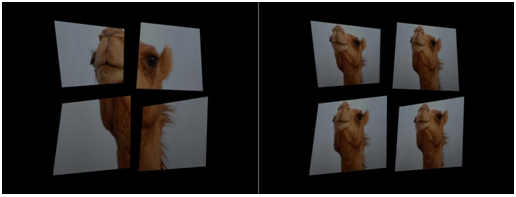
\includegraphics[width=0.7\textwidth]{./Cap5_vmt/vmtengine-maping.png}
  \caption[Imagen propia.]{Izquierda: Proyección plana. Derecha: Proyección por cara.}%imagen nuestra no hay que referenciar%
  \label{fig:VMT-Projection}
\end{figure}

La escena también contiene los efectos visuales que se ejecutarán durante el espectáculo. Estos efectos son la asignación de texturas en forma de imagen o video, ya sea a grupos de \emph{quads} u objetos tridimensionales, el \emph{fade}\footnote{Transición de un color inicial a uno final en un rango de tiempo.} en un material desde un color inicial a otro final, y la animación de la posición de un objeto tridimensional de un origen a un destino en un rango de tiempo.

El efecto de mapeo de texturas a pesar de ser básico es el más potente, pues permite lograr infinidad de resultados al momento de proyectar texturas sobre superficies, basando su complejidad en la creación de las texturas de imagen o video que se deseen utilizar. Al permitirse mapear estas texturas sobre objetos tridimensionales no es necesario distorsionar la forma de los videos generados sino que será \emph{VMT} quien los adaptará a la forma del objeto a mapear. El efecto \emph{fade} puede ser combinado en un objeto que ya disponga de una textura y así permitir por ejemplo su atenuación o resaltado.

A medida que trascurre la ejecución de los efectos se modifica sucesivamente la escena, y por lo tanto su estado en cada momento será el que resulte luego de la finalización de los efectos. Por ejemplo, si un objeto es de color rojo, y se le aplica un efecto \emph{fade} al azul su color luego de la ejecución del efecto continuará siendo azul.

Como se mencionó anteriormente, una de las tareas principales de \emph{VMT} es la representación en pantalla o proyección de los elementos gráficos. La implementación del dibujado se realiza en un bucle principal de la aplicación encargado de actualizar todos los objetos de la escena, procesar los eventos pendientes y finalmente desplegar el resultado.
Este es un proceso cíclico que se repite varias veces por segundo.
En cada uno de estos ciclos se generan los cuadros, también llamados \emph{frames}, que se muestran como resultado final.
Para dar la ilusión de continuidad la frecuencia de estos ciclos debe ser alta. En el caso de \emph{VMT}, ésta se limita a 60 ciclos por segundo aunque alcanzar esta frecuencia dependerá de varios factores como la cantidad de \emph{quads}, el tamaño de las texturas utilizadas y capacidad de procesamiento y memoria de los equipos.
Si esta frecuencia se encuentra muy por debajo de los 60 ciclos, la reproducción del espectáculo no será fluida y se podrán percibir saltos o pausas al ejecutarlo.
Para que esta frecuencia efectivamente se logre es necesario que el procesamiento de cada uno de los ciclos del bucle principal sea eficiente en cuanto al costo de procesamiento en cada tarea u operación. A continuación se muestra un pseudo-código del bucle principal de dibujado y se analizan cada una de las acciones que se toman, su impacto en cuanto al rendimiento del programa y las medidas que tomadas para su optimización:

\begin{algorithm}
    \caption{Pseudo-código bucle de dibujado.}
    \label{alg:mainLoop}
    \begin{algorithmic}
      \State $posicionarCamara();$
      \ForAll{objeto3d $obj$ en la escena}
        \ForAll{cara $c$ de $obj$}
             \State $mat = cargarMaterial(obj);$
             \State $c.dibujar(mat);$
         \EndFor
      \EndFor

      \State $resetCamara();$
      \ForAll {quad $q$ en la escena}
         \State $mat = q.cargarMaterial();$
         \State $q.dibujar(mat);$
      \EndFor
    \end{algorithmic}
\end{algorithm}

Un bucle de este estilo cuenta con varios cuellos de botella.
La carga de materiales implica copiar una textura a la zona de memoria de video correspondiente para utilizarla. Esto podría ser un proceso lento si no se disponen de las texturas precargadas en memoria. Es por esta razón que \emph{VMT} desde un comienzo carga las texturas en memoria y luego utiliza referencias para identificarlas y asociarlas a una unidad de textura de \emph{OpenGL}\footnote{www.opengl.org/wiki/Texture} para que se encuentre disponible al momento de ser utilizada.
Otra optimización realizada en la implementación de \emph{VMT} está en el uso de \emph{shaders} para el cálculo del resultado visual final. Los \emph{shaders} son ejecutados en la unidad de procesamiento gráfico (\emph{GPU}$^\dagger$) en forma paralela y por lo tanto son óptimos para ejecutar en bucles de este estilo.
La visualización fluida de un espectáculo de \emph{video mapping} es difícil de predecir ya que, como se puede ver en el pseudo-código, los tiempos de ejecución dependen de la cantidad de materiales, caras, objetos tridimensionales y \emph{quads} incluidos en la escena, así como también del hardware disponible.
Si se utilizan videos en las texturas, su compresión y resolución también afecta la fluidez del espectáculo. Preferentemente los videos deberían estar codificados con \emph{codecs} óptimos para ser utilizados en tiempo real. El mismo problema ocurre con formatos de imágenes comprimidas, pero teniendo un menor impacto en el rendimiento de la reproducción del espectáculo.

\subsection{Multi proyector}

Uno de los puntos fuertes de \emph{VMT} es la posibilidad de editar y visualizar un espectáculo de \emph{video mapping} utilizando más de un proyector.
Para brindar soporte a esto, \emph{VMT} fue diseñada con una arquitectura maestro-esclavo, implementada en dos componentes ejecutables de forma independiente.
El nodo maestro orquesta la reproducción del espectáculo enviando a los nodos esclavos instrucciones para la ejecución de los efectos. Estos nodos se pueden distribuir en varias computadoras, logrando la comunicación entre ellas mediante un protocolo de comunicación implementado utilizando \emph{Open Sound Control (OSC)}, estando a su vez este último construido sobre \emph{User Datagram Protocol (UDP$^\dagger$)}.
Los mensajes se componen por una cadena que lo identifica y un conjunto variable de parámetros que depende de cada mensaje en particular.
Dependiendo del tipo de mensaje, el nodo maestro decidirá si enviarlo a un nodo en particular, por ejemplo para el caso de operaciones sobre \emph{quads} ya que éstos se representan únicamente en un nodo, o enviarlo a todos los nodos al mismo tiempo, por ejemplo para operaciones sobre objetos tridimensionales ya que todas las cámaras tienen visibilidad sobre ellos.
Por la naturaleza del protocolo \emph{UDP}, es preferible contar con conexiones cableadas en lugar de inalámbricas dada la alta tasa de pérdida de paquetes que existe en este tipo de redes, lo cual podría causar desincronización de algunos nodos esclavos. \emph{OSC} también permite a cualquier aplicación capaz de enviar mensajes de este tipo y que conozca el formato de los mismos, controlar los esclavos y por consiguiente lo que se proyecta en los correspondientes proyectores.

La edición del espectáculo se realiza exclusivamente en el nodo maestro quien envía órdenes mediante el protocolo de comunicación a los nodos esclavos para que éstos representen objetos tridimensionales y \emph{quads}, aplicándoles efectos visuales.
En \emph{VMT}, los nodos se definen agregando cámaras virtuales que representan proyectores a la escena, asignando propiedades de ubicación para cada una en particular para luego definir la red de nodos esclavo con la información de conectividad necesaria y su correspondiente asociación al proyector conectado el nodo.

\begin{figure}[H]
  \centering
    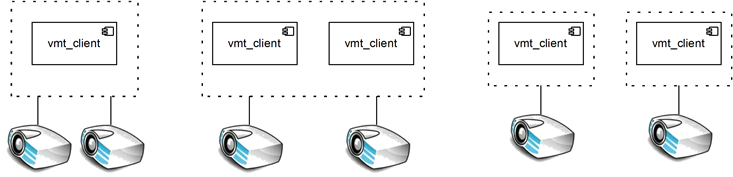
\includegraphics[width=0.8\textwidth]{./Cap5_vmt/vmt_multiProjector.png}
  \caption[Imagen propia.]{Escenarios posibles de múltiples proyectores en VMT}
  \label{fig:VMT-MultiProjector}
\end{figure}

El soporte de múltiples proyectores puede lograrse utilizando diferentes esquemas de distribución.
El más sencillo es el de conectar varios proyectores con más de una salida de video desde la misma computadora. Esto se logra mediante la utilización de una tarjeta de video con salidas múltiples, conectando cada proyector a cada una de estas salidas. Luego, se configura el sistema operativo para que extienda la resolución en las múltiples salidas y de esta forma se dispondrá de un área de trabajo mayor. Los diferentes sectores del área de trabajo serán desplegados por los proyectores conectados.
El componente esclavo de \emph{VMT} permite indicar al inicio de un espectáculo la resolución y la posición en pantalla en donde se desplegará. Controlando estos parámetros se permiten distintas variaciones en la configuración de la aplicación y en la disposición de los proyectores.
Esto también se puede lograr conectando dispositivos que dupliquen o tripliquen las salidas de video como las tarjetas \emph{DualHead2Go} o \emph{TripleHead2Go}\cite{Matrox} y de esta manera conectar dos o tres proyectores. El resultado es similar al anterior, extendiendo el área de trabajo a la resolución duplicada o triplicada, mediante el soporte del sistema operativo.
Estas variantes en la forma de conectar los proyectores son útiles cuando se desea proyectar sobre una superficie tan extensa que un único proyector no pueda abarcarla completamente, con la restricción de que los proyectores deben estar organizados de forma contigua.
En cambio, si queremos proyectar sobre zonas de la escena no contiguas entre si, lo ideal es contar con proyectores conectados a nodos distribuidos e independientes tanto al momento de la producción del espectáculo como al de su ejecución. Esto es posible explotando al máximo las posibilidades de distribución de \emph{VMT}, por ejemplo, ejecutando un nodo distinto en cada una de las computadoras distribuidas.

\subsection{Calibración}

\emph{VMT} tiene la capacidad de calibrar las cámaras virtuales para que la proyección reflejada por los proyectores se corresponda y ajuste a la geometría de la escena.
Como se mencionó anteriormente, \emph{VMT} permite trabajar simultáneamente de forma bidimensional y tridimensional, por lo tanto, cada uno de estos modos de trabajo requiere distintos mecanismos de calibración.

La calibración bidimensional se basa en ajustar los vértices de todos los \emph{quads} de una capa de forma conjunta.
Inicialmente, al preparar el modelo para el espectáculo, los \emph{quads} son posicionados en pantalla al mismo tiempo que estos son proyectados, cubriendo las áreas de interés a proyectar. Luego de este posicionamiento inicial, cualquier movimiento de los proyectores causará que se desajuste simultáneamente la proyección de todos los \emph{quads}. Si esto ocurriese, se hace necesario reposicionar los \emph{quads} para que vuelvan a cubrir las áreas a proyectar.
\emph{VMT} ofrece la posibilidad de ajustar todos los \emph{quads} pertenecientes a una misma capa de forma simultánea aplicando una homografía. Esta transformación es la que ocurre naturalmente en la proyección al variar la posición u orientación del mismo, por lo tanto es necesario aplicar la transformación inversa para que la proyección de los \emph{quads} se ajuste nuevamente a la superficie. La homografía queda definida conociendo cuatro puntos de origen y cuatro de destino, por lo que se puede calibrar la proyección escogiendo los cuatro vértices de un \emph{quad} y cuatro puntos en donde se desea proyectar dicho \emph{quad}.

Por otra parte, la calibración tridimensional se basa en hacer coincidir los parámetros de posición, orientación y proyección de las cámaras virtuales con los de los proyectores físicos. Este ajuste de parámetros se realiza manualmente por el usuario, utilizando las transformaciones de cámara explicadas anteriormente, \emph{dolly}, \emph{pan}, \emph{roll} y \emph{orbit}. Esta calibración es distinta para cada cámara virtual y proyector por lo que debe hacerse de forma independiente para cada uno de estos.

\section{Interfaz gráfica de usuario}

La interfaz gráfica de \emph{VMT} cuenta con ventanas y diálogos de altas, bajas y modificaciones para todos los tipos de objetos existentes en una escena. Fue diseñada en base a barras de herramientas flotantes de forma de tener visibilidad del editor tridimensional en todo momento sin ocupar áreas considerables del espacio de trabajo y poder observar así de mejor forma el impacto de las acciones realizadas.

\begin{figure}[H]
  \centering
    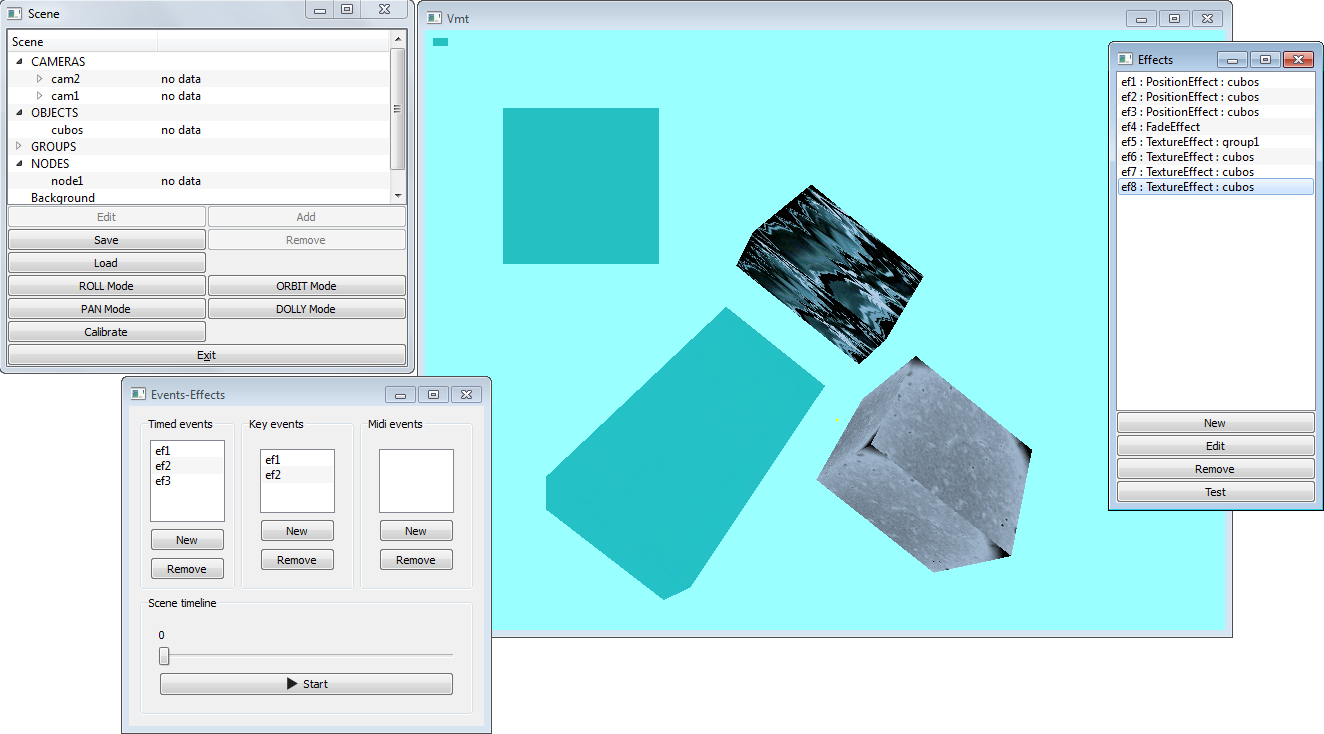
\includegraphics[width=0.8\textwidth]{./Cap5_vmt/vmt_todo.png}
  \caption[Imagen propia.]{Vista general de la interfaz de usuario de \emph{VMT}}
  \label{fig:VMT-MainWindow}
\end{figure}

Al inicio de la ejecución de \emph{VMT} se cuenta con una vista gráfica de la escena, un árbol con los elementos contenidos en la escena, la lista de definición de efectos y una línea de tiempo con las listas de efectos por tiempo, evento de teclado y \emph{MIDI}.
La ventana de escena brinda las funcionalidades principales de la aplicación, desde donde se manejan los objetos bidimensionales y tridimensionales, cámaras, capas y nodos distribuidos del espectáculo. También esta ventana ofrece los controles para la calibración de las cámaras virtuales para cambiar los modos de control ofrecidos.

\begin{figure}[H]
  \centering
    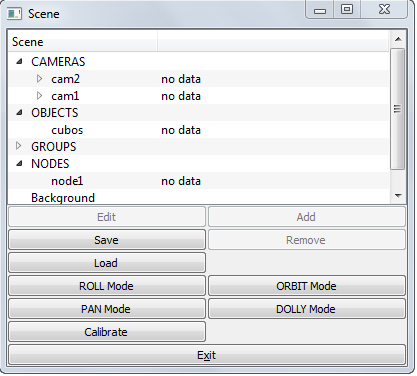
\includegraphics[width=0.5\textwidth]{./Cap5_vmt/vmt_scene.png}
  \caption[Imagen propia.]{Ventana para manejar la escena}
  \label{fig:VMT-SceneWindow}
\end{figure}

\subsection{Cámaras, capas y \emph{quads}}
Las cámaras virtuales tienen todas las propiedades usuales que se pueden encontrar en paquetes de software de animación tridimensional como son la posición, \emph{eye}, \emph{up}, \emph{FOV}, aspecto, \emph{near} y \emph{far}.
\emph{Eye}, \emph{up} y posición son ternas de coordenadas tridimensionales que identifican respectivamente hacia donde apunta la cámara, su dirección vertical y su punto de origen.
El parámetro \emph{FOV} o campo de vista, es el ángulo de apertura de la cámara virtual. A mayor ángulo de apertura, mayor cantidad de objetos serán incluidos en el campo visual de la cámara.
Por su parte el aspecto es un valor que representa la relación entre la resolución horizontal y vertical tanto de cámaras como de proyectores.
Finalmente, los parámetros \emph{near} y \emph{far}, son propios del modelo y no representan propiedades de los proyectores físicos. Éstos definen la distancia mínima y máxima de los objetos a la cámara, lo que será considerado para restringir la representación de los mismos.

\begin{figure}[H]
  \centering
    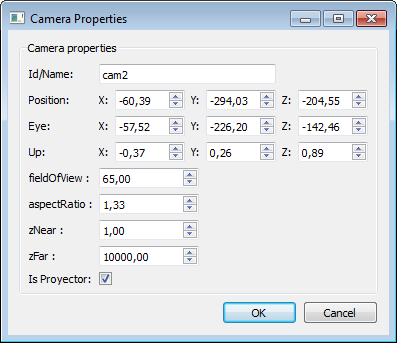
\includegraphics[width=0.5\textwidth]{./Cap5_vmt/vmt_cameraProperties.png}
  \caption[Imagen propia.]{Diálogo de propiedades de cámara}
  \label{fig:VMT-CameraProperties}
\end{figure}

Las cámaras virtuales en \emph{VMT} representan puntos de vista desde donde visualizar una escena tridimensional. Estas cámaras virtuales poseen la propiedad \emph{isProjector} que diferencia si esta cámara es utilizada para representar el punto de vista de un proyector o un punto de vista arbitrario. La aplicación utiliza esta información para asociar las cámaras que representen proyectores a los nodos esclavos en una configuración multiproyector.

\begin{figure}[H]
  \centering
    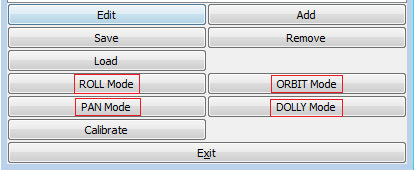
\includegraphics[width=0.5\textwidth]{./Cap5_vmt/vmt_SceneBotonera.png}
  \caption[Imagen propia.]{Acciones para seleccionar modo de movimiento de la cámara activa}
  \label{fig:VMT-CameraActions}
\end{figure}

Una vez seleccionado el modo de la cámara, arrastrando el ratón manteniendo presionado el botón izquierdo se mueve la cámara de manera acorde al modo seleccionado.
Cada cámara es a su vez un contenedor de capas, cuyo propósito es manejar todo lo relacionado al mapeo sobre estructuras bidimensionales. Por esta razón, las capas son a su vez contenedores de \emph{quads} sobre los cuales se realizan todas las operaciones y efectos disponibles.

\begin{figure}
	\begin{center}
		\begin{tabular}[c]{cc}
			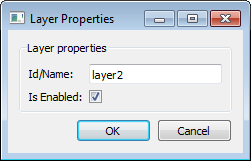
\includegraphics[width=0.3\textwidth]{./Cap5_vmt/vmt_layerProperties.png}
				&        
			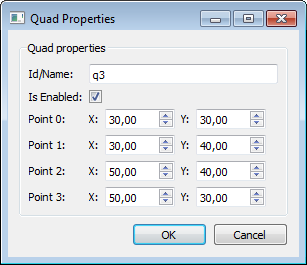
\includegraphics[width=0.3\textwidth]{./Cap5_vmt/vmt_quadProperties.png}
		\end{tabular}
	\end{center}
	\caption[Imagen propia.]{Propiedades de los objetos capa y \emph{Quad}}
	\label{fig:VMT-LayerQuadProperties}
\end{figure}

Tanto \emph{quads} como capas tienen propiedades que pueden ser modificadas en tiempo de edición para mostrarse u ocultarse completamente. Si se oculta una capa, todos los \emph{quads} contenidos en ella también se ocultarán. En caso de revelarla, todos los \emph{quads} visibles volverán a desplegarse.

\subsection{Objetos tridimensionales}

\emph{VMT} permite el manejo de objetos tridimensionales, importándolos de archivos con formato de malla triangular de tipo \emph{3DS}.
Fue escogido este formato debido a que es un estándar utilizado por los programas de modelado tridimensional más populares, y por la disponibilidad de bibliotecas facilitan su manipulación.
Como se mencionó anteriormente, la edición de los objetos tridimensionales se delega a aplicaciones para este propósito, limitándose \emph{VMT} a su posicionamiento.

\begin{figure}[H]
  \centering
    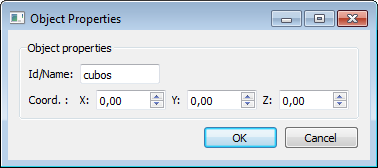
\includegraphics[width=0.5\textwidth]{./Cap5_vmt/vmt_objectProperties.png}
  \caption[Imagen propia.]{Diálogo de propiedades de objeto tridimensional}
  \label{fig:VMT-ObjectProperties}
\end{figure}

\subsection{Efectos}

Se proveen ventanas flotantes tanto para la definición de efectos como para la asociación con sus disparadores como ser un instante específico, un evento de teclado o un evento \emph{MIDI}.
Si un efecto es definido para ser desplegado en un instante dado, éste se podrá visualizar durante el transcurso de la línea de tiempo. En caso de ser definido por evento de teclado o \emph{MIDI}, éste será ejecutado cada vez que el evento asociado suceda.

El efecto de posición de objetos tridimensionales permite animar el objeto trasladándolo de una posición inicial a una final en un rango de tiempo.

\begin{figure}[H]
  \centering
    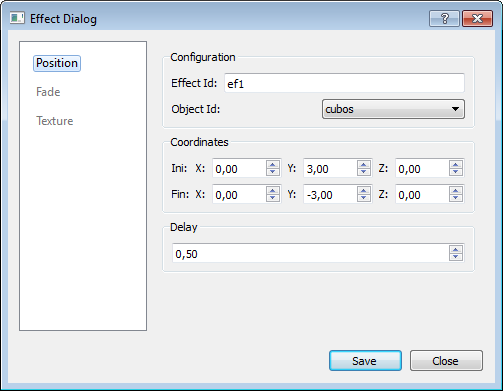
\includegraphics[width=0.5\textwidth]{./Cap5_vmt/vmt_EfectDialog1.png}
  \caption[Imagen propia.]{Diálogo de definición de efecto de tipo posición}
  \label{fig:VMT-EffectPossition}
\end{figure}

El efecto \emph{fade} es aplicable a grupos de \emph{quads} y permite colorear todos los \emph{quads} del grupo variando desde un color inicial y pasando por toda la gama de colores intermedios hasta llegar al color final en un rango de tiempo. Para la selección de colores se utiliza un diálogo específico para este propósito.

\begin{figure}[H]
  \centering
    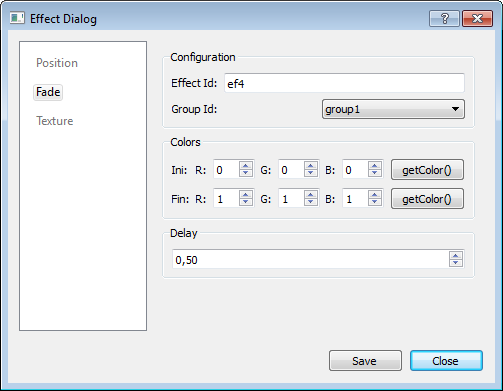
\includegraphics[width=0.5\textwidth]{./Cap5_vmt/vmt_EfectDialog2.png}
  \caption[Imagen propia.]{Diálogo de definición de efecto de tipo \emph{fade}}
  \label{fig:VMT-EffectFade}
\end{figure}

Los efectos de tipo textura son aplicables tanto a grupos de \emph{quads} como a objetos tridimensionales, definiendo texturas de tipo imagen o video. En ambos casos es necesario proporcionar la ruta al archivo multimedia correspondiente. Para el caso específico de un efecto de textura asociado a un objeto tridimensional, es necesario proporcionar además la cara o conjunto de caras sobre los cuales se mapeará dicho efecto. Este conjunto de caras se representa en el formato \emph{3DS} asociándole un material, para luego identificarlas mediante su nombre.

\begin{figure}[H]
  \centering
    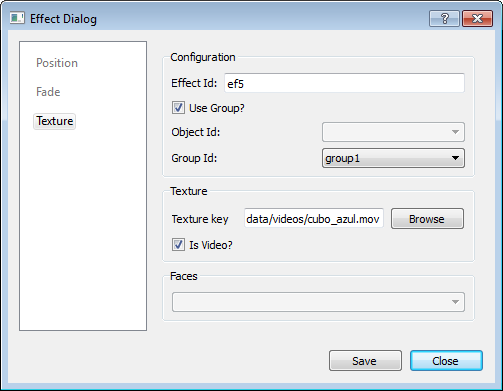
\includegraphics[width=0.5\textwidth]{./Cap5_vmt/vmt_EfectDialog3.png}
  \caption[Imagen propia.]{Diálogo de definición de efecto de tipo textura}
  \label{fig:VMT-EffectTexture}
\end{figure}

\begin{figure}[H]
  \centering
    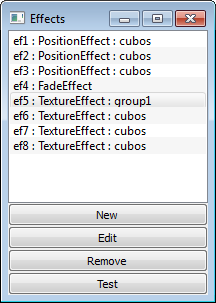
\includegraphics[width=0.2\textwidth]{./Cap5_vmt/vmt_Efects.png}
  \caption[Imagen propia.]{Lista de efectos definidos en la escena}
  \label{fig:VMT-EffectList}
\end{figure}

Es posible visualizar el efecto que se está creando presionando el botón \emph{Test} de la lista de efectos. Esto disparará la ejecución del efecto seleccionado por una única vez.

\subsection{Calibración}

El proceso de calibración en \emph{VMT} se basa en posicionar cuatro puntos de la superficie donde se proyecta y cuatro puntos de la capa contenedora de \emph{quads} para de esta forma calcular la matriz de transformación de la homografía que los hace corresponder.

\begin{figure}[H]
  \centering
    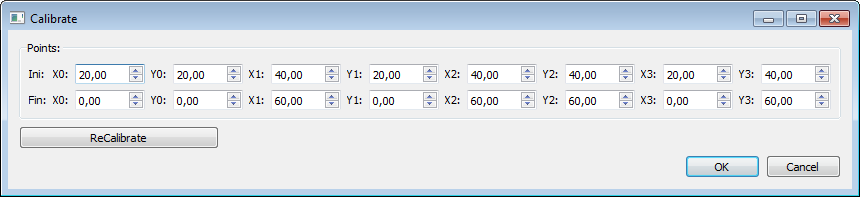
\includegraphics[width=0.6\textwidth]{./Cap5_vmt/vmt_Calibrate.png}
  \caption[Imagen propia.]{Diálogo para configurar y ejecutar la calibración}
  \label{fig:VMT-Calib}
\end{figure}

Al ingresar en el modo calibración se muestran en la pantalla de edición cuatro puntos azules de destino y cuatro puntos rojos de origen junto con el diálogo de configuración de la calibración.
El diálogo posee controles para posicionar cada uno de los ocho puntos mostrados en pantalla. Se deberán posicionar los cuatro puntos de origen en regiones significativas de la capa donde hayan vértices de \emph{quads}, preferiblemente alejados entre si para de esta forma minimizar el error obtenido al calcular la matriz.
Los cuatro puntos de destino se deberán posicionar observando la proyección de estos sobre la superficie, trasladándolos hasta que coincidan con la superficie que se desea cubrir. Una vez que los ocho puntos estén posicionados se podrá calcular y aplicar la nueva matriz de calibración confirmando con el botón \emph{OK}.
Mediante el botón \emph{ReCalibrate} se reestablece la calibración original, descartando los cambios realizados.

\subsection{Línea de tiempo}

Tanto para las fases de producción y previsualización del espectáculo como para su reproducción en vivo, es necesario contar con controles para el manejo de la línea de tiempo.

\begin{figure}[H]
  \centering
    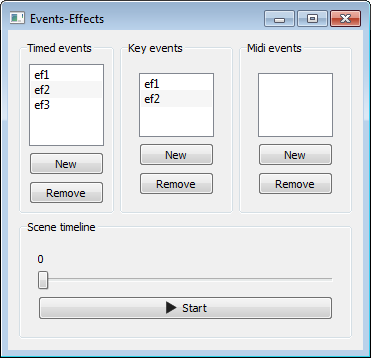
\includegraphics[width=0.5\textwidth]{./Cap5_vmt/vmt_events_effects.png}
  \caption[Imagen propia.]{Diálogo con línea de tiempo y lista de efectos asociados a tiempo y eventos}
  \label{fig:VMT-Timeline}
\end{figure}

La aplicación permite iniciar la ejecución de la línea de tiempo mediante el botón \emph{Start}. Se provee una vista gráfica representada con una barra deslizante y una vista numérica para reflejar el avance en el tiempo en relación a la duración total del evento.
Utilizando la barra deslizante es posible navegar por la línea de tiempo e iniciar la visualización del espectáculo desde cualquier instante deseado. Esto último es muy útil para la fase de producción del espectáculo en la cual es muy común que el usuario se quiera concentrar en un lapso específico en el que se está trabajando.
El diálogo contiene los efectos asociados a eventos agrupados por tipo, pudiendo estos referenciar un instante dado, un evento de teclado o proveniente de dispositivos de entrada \emph{MIDI}.

\subsection{Nodos remotos}

Para modelar la red de nodos esclavos de \emph{VMT} en los cuales se conectarán proyectores remotos es preciso definir para cada uno de ellos, su dirección \emph{IP} y número de puerto en donde estarán configurados así como también la cámara definida en la escena que representará al proyector asociado.

\begin{figure}
	\begin{center}
		\begin{tabular}[c]{cc}
			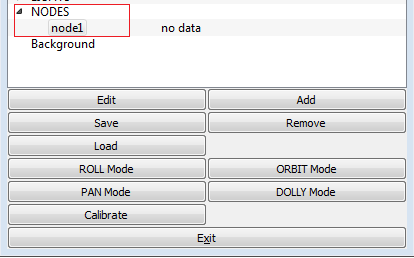
\includegraphics[width=0.3\textwidth]{./Cap5_vmt/vmt_nodeProperties_1.png}
				&
			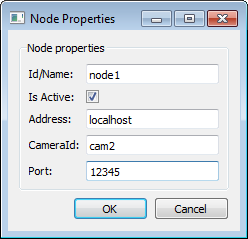
\includegraphics[width=0.3\textwidth]{./Cap5_vmt/vmt_nodeProperties_2.png}
		\end{tabular}
	\end{center}
	\caption[Imagen propia.]{Lista de nodos y diálogo de propiedades de nodos}
	\label{fig:VMT-Nodes}
\end{figure}

\subsection{Escena en XML}
El almacenamiento de la escena y su carga se realiza mediante archivos \emph{XML} estándar.
La interfaz provee diálogos específicos para guardar y cargar estos archivos.

\begin{figure}[H]
  \centering
    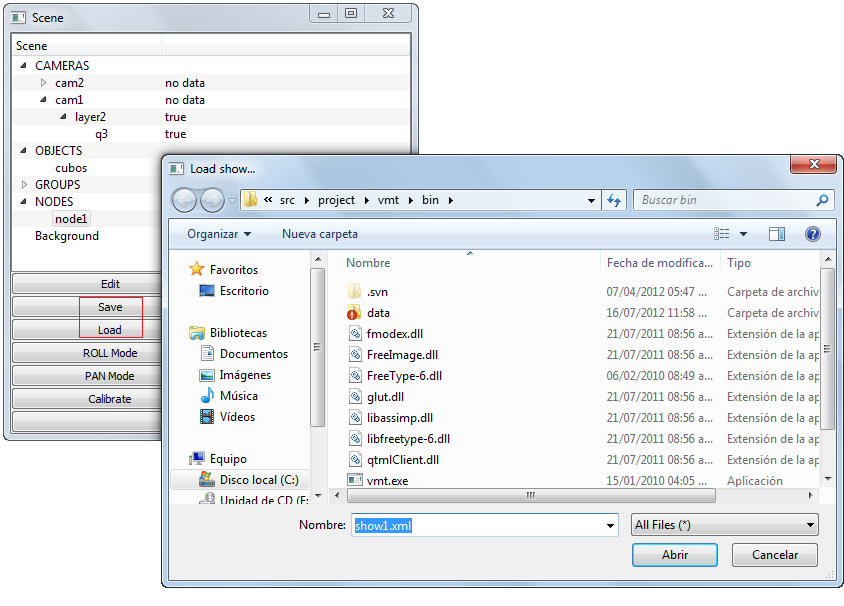
\includegraphics[width=0.5\textwidth]{./Cap5_vmt/vmt_loadShow.png}
  \caption[Imagen propia.]{Diálogo para cargar y guardar archivos \emph{XML}.}
  \label{fig:VMT-XML}
\end{figure}

\subsection{Decisiones de implementación de la interfaz gráfica de usuario}
Para la implementación del módulo de interfaz gráfica se utilizó \emph{Qt Framework}\cite{Qt-framework} como biblioteca de base para la creación de las ventanas, controles gráficos y manejo de la comunicación que ocurre entre las ventanas y los modelos de \emph{VMT}. Esta biblioteca utiliza el patrón de diseño \emph{Model-View-Controller (MVC)}\cite{QTMVC}, lo que exige generar para cada ventana, modelos que manejan sus datos relevantes.
Se hizo uso de la funcionalidad para internacionalización de las interfaces gráficas, las que por el momento están tomando valores por defecto en idioma inglés. \emph{Qt Framework} es multiplataforma y puede ser utilizado en varios de los sistemas operativos más populares como \emph{Linux}, \emph{Mac OS X} y \emph{Windows}, por esta razón es que fue escogido como base para el módulo de interfaz gráfica.

\section{Prototipo de calibración tridimensional}
En el marco de este proyecto se desarrolló un prototipo de calibración basado en un método cuyo objetivo es obtener la posición del proyector con respecto a un sistema de coordenadas ubicado en un punto relativo a la escena. Para ello se utiliza una superficie plana de calibración que puede existir ya en la escena o puede ser ubicada sobre ésta de forma temporal. Esta superficie de calibración deberá ser un plano rectangular en donde uno de los vértices será el centro de coordenadas que se desea determinar. La orientación del plano determinará la alineación del centro de coordenadas con sus ejes $X$ e $Y$ alineados con dos de los bordes del plano y el eje $Z$ perpendicular a éste.
Se utiliza además un proyector el cual es representado mediante el modelo \emph{pinhole}.

Para encontrar el sistema de coordenadas buscado, se resuelve el problema opuesto que es encontrar la posición del punto que será origen del nuevo centro de coordenadas con respecto al centro de proyección ubicado dentro del proyector. Este método utiliza tres de los vértices de la superficie de calibración que formarán una base del nuevo sistema de coordenadas. Las medidas de la superficie de calibración son conocidas por lo que las distancias entre sus vértices también lo son. Desde el centro del proyector se proyectan rayos de luz, tres de los cuales pasan por los vértices de la superficie de calibración y también por el centro de proyección con coordenadas $(0, 0, 0)$. Para obtener la ecuación de estos rayos se precisa únicamente un punto distinto del origen. La ecuación de este punto puede ser obtenida utilizando las coordenadas en pantalla del píxel que se proyecta en cada vértice de la superficie de calibración.

\begin{figure}[H]
  \centering
    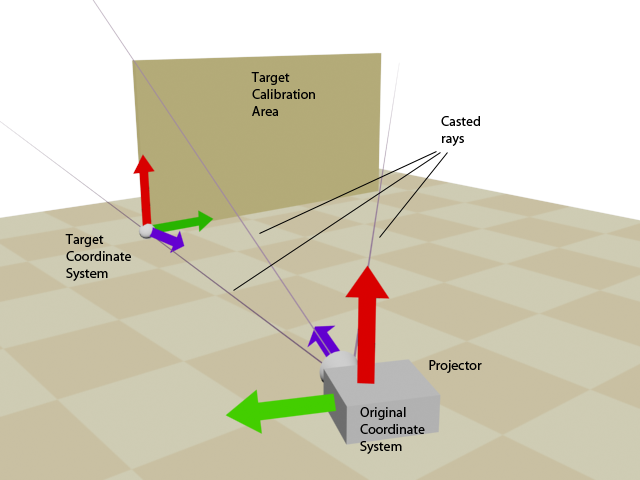
\includegraphics[width=0.7\textwidth]{./Cap2_videomapping/CalibrationSketch}
  \caption[Imagen propia.]{Esquema de calibración.}
  \label{fig:CalibrationSketch}
\end{figure}

Usando las coordenadas en la pantalla de estos puntos junto con los parámetros intrínsecos del proyector que son su resolución y ángulo de proyección, es posible encontrar las coordenadas del punto con respecto al centro de proyección y por tanto la ecuación del rayo.
\[
a(t) = \vec{P} . t,	\mbox{ ecuación del rayo en dónde } \vec{P} \mbox{ es cualquier punto del rayo.}
\]
\[
\begin{cases}
P(X) = \frac{res_x}{2} - s_x \\
P(Y) = \frac{res_y}{2} - s_y \\
P(Z) = \frac{res_y}{2 \cdot \tan \frac{fov_y}{2}}
\end{cases}
\]
en donde $s_x$ y $s_y$ son las coordenadas del píxel, $res_x$ y $res_y$ son la resolución horizontal y vertical del proyector y $fov_y$ es el ángulo de proyección vertical del proyector.

Aplicando esta ecuación a cada uno de los puntos a determinar se obtienen las ecuaciones paramétricas de los tres rayos. Vale aclarar que estos puntos $P$ son puntos de los rayos pero no necesariamente coinciden con los vértices de la superficie de calibración. Resta hallar las coordenadas de los vértices determinando el parámetro $t$ para cada ecuación. Para hallar este parámetro se resuelve un sistema de ecuaciones utilizando las tres ecuaciones de los rayos y las distancias conocidas entre estos puntos.
% Sistema de ecuaciones %
\[
\begin{cases}
\lVert{a(t_0) - b(t_1)} = j\rVert \\
\lVert{b(t_1) - c(t_2)} = k\rVert \\
\lVert{c(t_2) - a(t_0)} = l\rVert
\end{cases}
\]
siendo $a$, $b$ y $c$ los rayos y $j$, $k$ y $l$ las distancias entre las parejas de puntos.
La solución será entonces los parámetros $t_0$, $t_1$ y $t_2$ que satisfacen el sistema de ecuaciones no lineal.
Una aproximación a esta solución se puede obtener utilizando métodos numéricos, por ejemplo, el método \emph{trust-region-dogleg}\cite{TrustRegionDogleg}.
Una vez hallados los valores para $t_0$, $t_1$ y $t_2$, las coordenadas de los vértices de la superficie de calibración son $a(t_0)$, $b(t_1)$ y $c(t_2)$.
La base para el sistema de coordenadas con origen en el punto $P$ es:
\[
x' = \frac{b(t_1) - a(t_0)}{\lVert b(t_1) - a(t_0) \rVert},\quad y' = \frac{c(t_2) - a(t_0)}{\lVert c(t_2) - a(t_0)\rVert},\quad z' = -x' \times y'
\]
La ubicación del proyector en este nuevo sistema se obtiene proyectando cualquiera de los rayos en la nueva base de coordenadas.

\section{Tratamiento de malla}

Para generar mallas que puedan ser manejadas por \emph{VMT} se desarrolló separadamente una aplicación que recibe como entrada una nube de puntos a procesar.
Como salida se generan mallas triangulares en el formato estándar \emph{OBJ}.

Para la implementación de este módulo se utilizan los algoritmos descriptos en el capítulo de estado del arte, incluidos en \emph{VcgLib} y que forman parte del procesamiento de malla propuesto. Para visualizar y evaluar los resultados esperados fue utilizada la aplicación de código abierto para la manipulación de mallas tridimensionales en diferentes formatos \emph{MeshLab}\cite{MeshLab}. Particularmente se utilizan los algoritmos de muestreo \emph{Poisson-disk} para reducir y normalizar los puntos de la malla inicial, \emph{normal extrapolation} para el cálculo de normales y reconstrucción de superficies de Poisson para la reconstrucción de la malla final.

Esta aplicación cuenta con una sencilla interfaz de usuario, con una única ventana que recibe los parámetros para la configuración de los algoritmos que se ejecutan en cada uno de los pasos del procesamiento.

\begin{figure}[H]
  \centering
    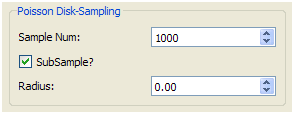
\includegraphics[width=0.5\textwidth]{./Cap2_videomapping/malla-poissongui.png}
  \caption[Imagen propia.]{Configuración de parámetros del algoritmo \emph{Poisson-disk}}
  \label{fig:Mesh-PoissonGui}
\end{figure}

\begin{figure}[H]
  \centering
    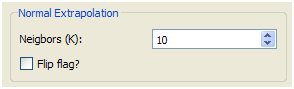
\includegraphics[width=0.5\textwidth]{./Cap2_videomapping/malla-normalextrapolation.png}
  \caption[Imagen propia.]{Configuración de parámetros para reconstrucción de normales}
  \label{fig:Mesh-Extrapolation}
\end{figure}

\begin{figure}[H]
  \centering
    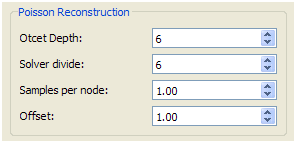
\includegraphics[width=0.5\textwidth]{./Cap2_videomapping/malla-poissonreconstruction.png}
  \caption[Imagen propia.]{Configuración de parámetros para reconstruccion de malla de Poisson}
  \label{fig:Mesh-Normals}
\end{figure}

\subsection{Pruebas y resultados}

Para validar el correcto funcionamiento de esta técnica mediante los tres algoritmos descritos, fue utilizada una malla inicial de 5021 vértices y 9608 caras triangulares. Cabe destacar que si bien se ha mencionado que la malla de entrada debe ser simplemente una nube de puntos, se pueden utilizar mallas con caras, aunque estas serán ignoradas e incluso eliminadas de la malla de salida del primer paso del procesamiento (muestreo de \emph{Poisson-disk}).
Luego de experimentar con varios juegos de datos iniciales durante varias ejecuciones del procesamiento, se fijaron de manera personalizada para la malla de entrada algunos parámetros clave. Dado que la muestra inicial tiene alrededor de 5000 puntos, fueron elegidas 5000 muestras para el algoritmo de \emph{Poisson-disk}. Luego, para la extrapolación de normales se utilizan $K=15$ vecinos para la toma de decisiones locales de aproximación.
La aplicación de estos algoritmos resultó ser lo esperado en términos estructurales de cada malla procesada en cada uno de los pasos.

\begin{table}
\begin{center}
\begin{tabular}{|l||cc|} \hline
  Fase & Vértices & Caras \\
  Nube inicial & 5021 & 9608 \\
  Poisson-disk & 1776 & 0 \\
  Extrapolación Normales & 1776 & 0 \\
  Reconstrucción de Poisson & 1959 & 3910 \\ \hline %hay 1959 puntos en lugar de 1776, por que?%
\end{tabular}
\caption{Comparación de estructura de mallas de entrada y salida en cada fase}
\end{center}
\end{table}

\begin{figure}[H]
  \centering
    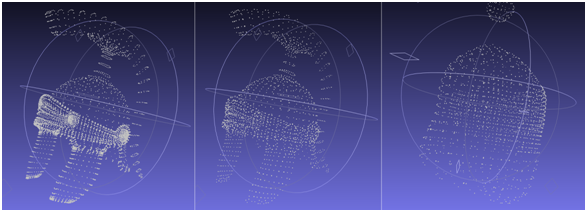
\includegraphics[width=0.8\textwidth]{./Cap2_videomapping/malla-nubepuntos.png}
  \caption[Captura de Meshlab http://meshlab.sourceforge.net]{1) Nube de puntos inicial con 5021 vértices. 2) Resultado de muestreo \emph{Poisson-disk} con 1776 vértices. 3) Luego de extrapolar normales y reconstruir la malla con 1959 vértices y 3910 caras.}
  \label{fig:Mesh-Results}
\end{figure}
 